\section{Neural Networks}

Success in learning crucially depends on the quality of the features. The key idea of neural networks is to parameterize the feature maps and optimize over the parameters.

We want to build a complex model out of simple components:
$$\phi(x, \theta) = \varphi(\theta^\top x)$$

Hereby, $\theta \in \R^d$ are the weights and $\varphi: \R \mapsto \R$ is a nonlinear \textbf{activation function}. Possible activation functions are:
\begin{itemize}
	\item \textbf{Identity}: $\varphi(z) = z$
	\item \textbf{Sigmoid}: $\varphi(z) = \frac{1}{1 + \exp(-z)}$
	\item \textbf{Tanh}: $\varphi(z) = \tanh z = \frac{\exp(z) - \exp(-z)}{\exp(z) + \exp(-z)}$
	\item \textbf{ReLU}: $\varphi(z) = \max (0,z)$
\end{itemize}

Nesting these components we create networks of the form:

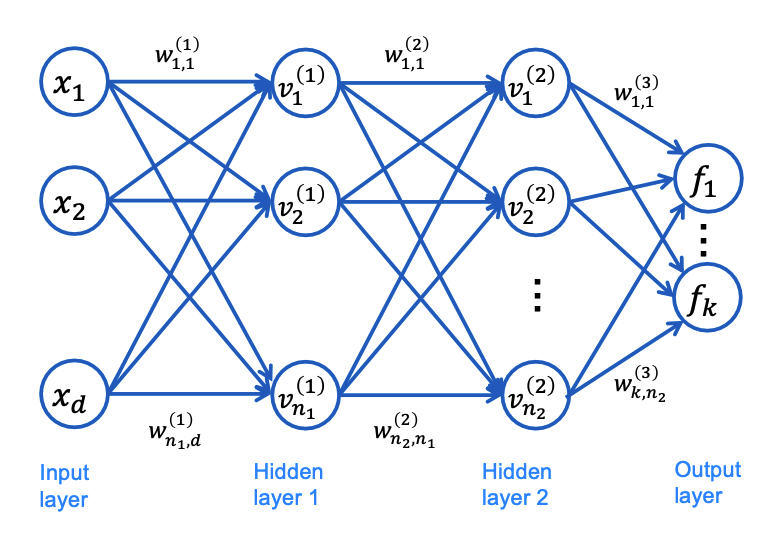
\includegraphics[width=\columnwidth]{neural-network.png}

Where $v_i = \varphi(z_i)$ and $z_i$ is the sum of inputs times their weight. To deal with biases we introduce a "constant" 1 feature to each layer. Note that we can have as many layers as we want and use different activation functions per layer. Such networks are typically trained via SGD.

By the universal approximation theorem, we can approximate any arbitrary smooth target function, given at least one layer with sufficient width.

\subsection{Forward Propagation}

This is the process of calculating the output for a given input.
\begin{itemize}
	\item For input layer 
		  $$v^{(0)} = [x; 1]$$
	\item For each hidden layer $1:L-1$
		  $$z^{(l)} = W^{(l)} v^{(l-1)} \quad \text{ and } \quad v^{(l)} = [\varphi(z^{(l)}); 1]$$
	\item For output layer
		  $$f = W^{(L)} v^{(L-1)}$$
\end{itemize}

\subsection{Backpropagation}

We can use the loss functions we already know to compute the loss. For multi output networks, we use the sum of per-output for regression tasks and cross-entropy loss for classification tasks. As mentioned we use SGD to fit our neural network. We want to jointly optimize over all weight for all layers. This is generally a non-convex optimization problem. Nevertheless, we can try to find a local optimum. In order to apply SGD, need to compute $\nabla_W \ell(W; x, y)$ w.r.t. each weight $w_{i,j}^{(l)}$:

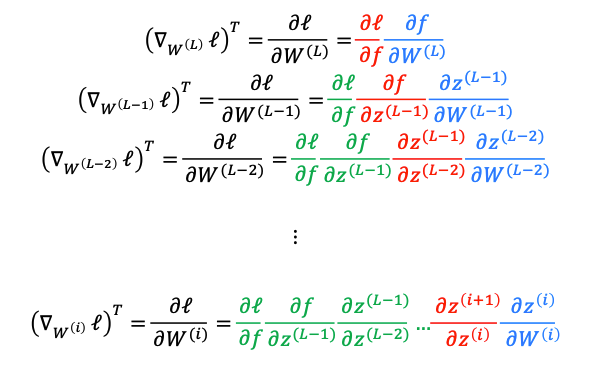
\includegraphics[width=\columnwidth]{backpropagation.png}

Notice that we can reuse calculations from \color{ForestGreen} \textbf{the previous layer} \color{Black}, \color{ProcessBlue} \textbf{forwards pass} \color{Black} and only have to compute \color{Red} \textbf{the gradient} \color{Black} for each layer.

Since the optimization problem is non-convex the initialization of the weights matters. With inappropriate weights we can run into exploding or vanishing gradients. To avoid this we randomly initialize the weights based on some distribution assumption for the activation function.

\subsection{Overfitting}

Since any deep neural network has a lot more parameters then data points to train on, overfitting can happen easily. To avoid this we use:
\begin{itemize}
	\item \textbf{Regularization}: add a penalty on the weights to the cost function
	\item \textbf{Early Stopping}: stop training once validation error stop to decrease
	\item \textbf{Dropout}: randomly ignore hidden units during training with probability $p$, after training all units are used and weights are multiplied by $p$
	\item \textbf{Batch Normalization}: normalize the input data (mean 0, variance 1) in each layer
\end{itemize}

\subsection{Convolutional Neural Networks}

CNN are a specialized architecture for neural networks. The idea is that predictions should be unchanged under some transformations of the data, e.g. rotation of images.

\begin{center}
	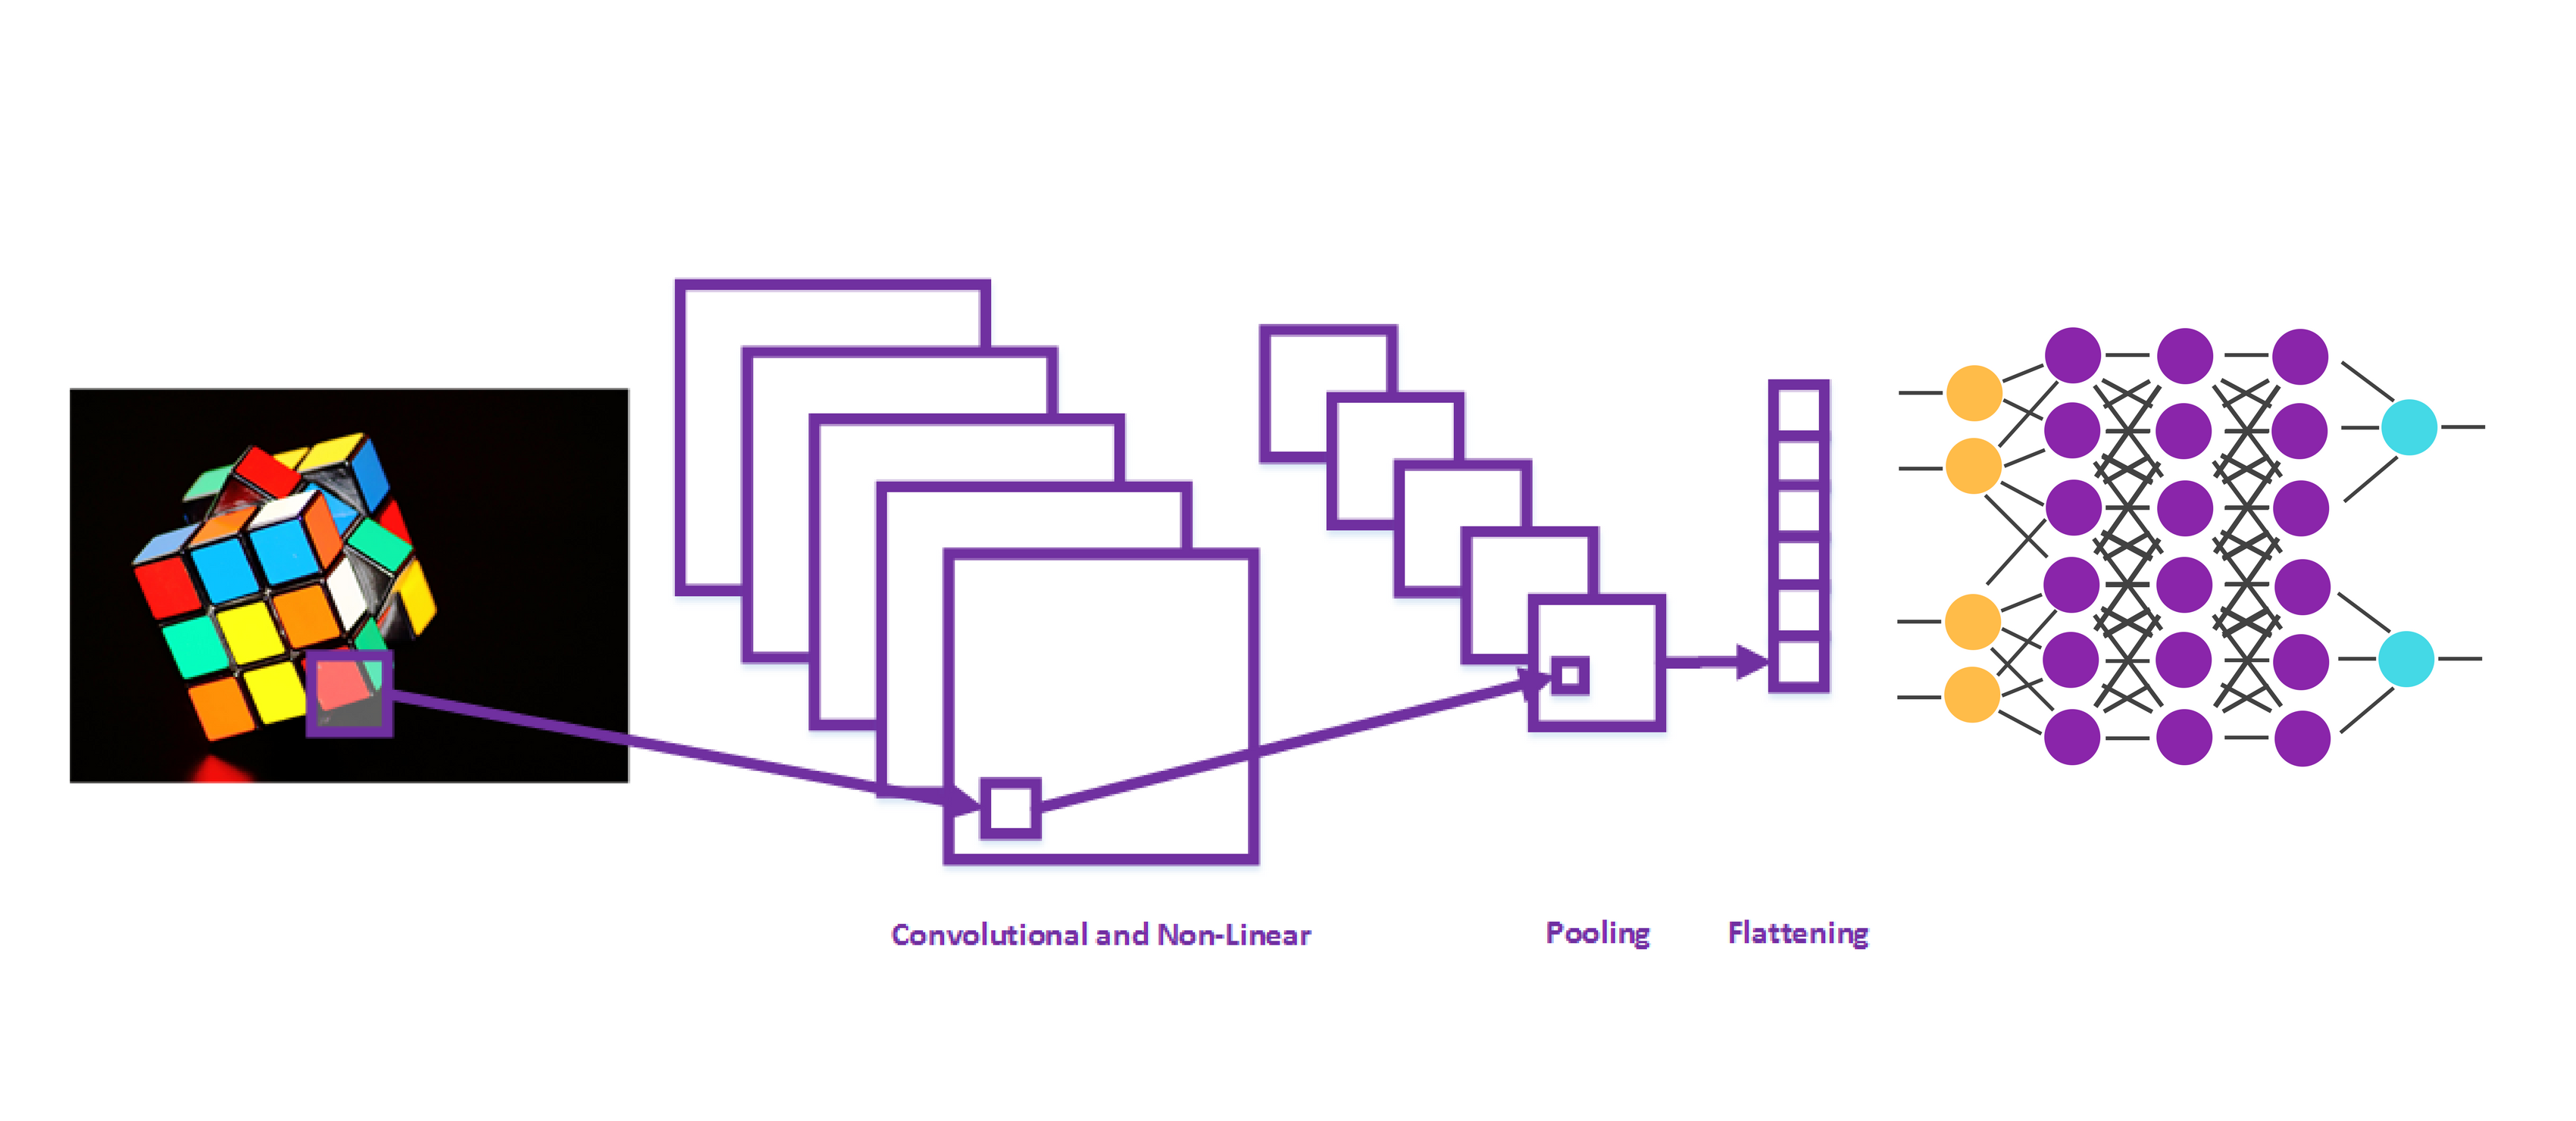
\includegraphics[width=\columnwidth]{cnn.png}
\end{center}

Each layer is not fully connected but structured. The activation function is applied to the element-wise convolution:
$$\varphi(W * v^{(l)})$$

The output dimension when applying $m$ different $f \times f$ filters to an $n \times n$ image with padding $p$ and stride $s$ is:
$$l = \frac{n + 2p - f}{s} + 1$$

Additionally we might use average or max pooling layers to aggregate several units into a single one, or use stride layers to skip units to decrease size.

\begin{center}
	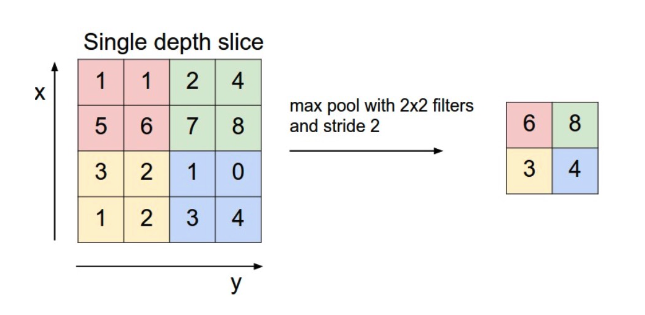
\includegraphics[width=\columnwidth]{pooling.png}
\end{center}

